\documentclass{article}
\usepackage[top=1cm, bottom=1cm, left=1.5cm, right=1.5cm]{geometry} % Reduced margins
\usepackage{graphicx}
\usepackage{listings}
\usepackage{hyperref}
\usepackage{float}
\usepackage{tcolorbox}
\tcbuselibrary{listings,breakable}

\title{Verilog Design Report: Convolution, Adder, and Ripple Carry Adder}
\author{Dhawal(EE24BTECH11015)}
\date{\today}

\begin{document}

\maketitle

\section{Question 1: 8-Element Vector Convolution Module}

\subsection{Detailed Approach}
\begin{enumerate}
    \item The convolution module computes the discrete linear convolution of two 8-element vectors.
    \item Input vectors x and h are each 4-bit wide (8 elements total).
    \item The output has 16 elements (8+8-1) due to convolution properties.
    \item Each output element y[n] is calculated as the sum of products of x[k] and h[n-k].
    \item The implementation uses combinatorial logic with an always @(*) block.
    \item Temporary 8-bit registers store intermediate results before truncation.
    \item The design performs parallel multiplications and additions for each output tap.
    \item Output is truncated to 4 bits by taking only the lower nibble of each result.
    \item No pipelining is implemented - this is a purely combinatorial design.
    \item The module demonstrates direct implementation of convolution formula without optimization.
\end{enumerate}

\subsection{Code Explanation}
Key points about the implementation:
\begin{itemize}
    \item Input vectors are split into individual 4-bit elements (x0-x7, h0-h7)
    \item 16 output elements (y0-y15) cover all possible convolution results
    \item Temporary 8-bit registers prevent overflow during intermediate calculations
    \item Combinatorial always block calculates all outputs simultaneously
    \item Each output is the sum of relevant input products
    \item Final assignments truncate results to 4 bits
    \item No clock or reset needed - pure combinational logic
    \item Simple direct implementation of convolution formula
\end{itemize}

\begin{tcolorbox}[title=Convolution Module Code, breakable]
\begin{lstlisting}[language=Verilog]
module convolution (
    input  [3:0] x0, x1, x2, x3, x4, x5, x6, x7,
    input  [3:0] h0, h1, h2, h3, h4, h5, h6, h7,
    output [3:0] y0, y1, y2, y3, y4, y5, y6, y7,
                 y8, y9, y10, y11, y12, y13, y14, y15
);
    reg [7:0] temp0, temp1, temp2, temp3, temp4, 
    temp5, temp6, temp7;
    reg [7:0] temp8, temp9, temp10, temp11, 
    temp12, temp13, temp14, temp15;

    always @(*) begin
        temp0  = (x0 * h0);
        temp1  = (x0 * h1) + (x1 * h0);
        temp2  = (x0 * h2) + (x1 * h1) + (x2 * h0);
        temp3  = (x0 * h3) + (x1 * h2) + (x2 * h1) + (x3 * h0);
        temp4  = (x0 * h4) + (x1 * h3) + (x2 * h2) + (x3 * h1) + (x4 * h0);
        temp5  = (x0 * h5) + (x1 * h4) + (x2 * h3) + (x3 * h2) + (x4 * h1) 
        + (x5 * h0);
        temp6  = (x0 * h6) + (x1 * h5) + (x2 * h4) + (x3 * h3) + (x4 * h2) 
        + (x5 * h1) + (x6 * h0);
        temp7  = (x0 * h7) + (x1 * h6) + (x2 * h5) + (x3 * h4) + (x4 * h3) 
        + (x5 * h2) + (x6 * h1) + (x7 * h0);
        temp8  = (x1 * h7) + (x2 * h6) + (x3 * h5) + (x4 * h4) + (x5 * h3) 
        + (x6 * h2) + (x7 * h1);
        temp9  = (x2 * h7) + (x3 * h6) + (x4 * h5) + (x5 * h4) + (x6 * h3) 
        + (x7 * h2);
        temp10 = (x3 * h7) + (x4 * h6) + (x5 * h5) + (x6 * h4) + (x7 * h3);
        temp11 = (x4 * h7) + (x5 * h6) + (x6 * h5) + (x7 * h4);
        temp12 = (x5 * h7) + (x6 * h6) + (x7 * h5);
        temp13 = (x6 * h7) + (x7 * h6);
        temp14 = (x7 * h7);
        temp15 = 0;
    end

    assign y0  = temp0[3:0];
    assign y1  = temp1[3:0];
    assign y2  = temp2[3:0];
    assign y3  = temp3[3:0];
    assign y4  = temp4[3:0];
    assign y5  = temp5[3:0];
    assign y6  = temp6[3:0];
    assign y7  = temp7[3:0];
    assign y8  = temp8[3:0];
    assign y9  = temp9[3:0];
    assign y10 = temp10[3:0];
    assign y11 = temp11[3:0];
    assign y12 = temp12[3:0];
    assign y13 = temp13[3:0];
    assign y14 = temp14[3:0];
    assign y15 = temp15[3:0];
endmodule
\end{lstlisting}
\end{tcolorbox} 

\subsection{Testbench}
Key testbench features:
\begin{itemize}
    \item Tests three different input scenarios
    \item Includes basic, impulse, and max-value test cases
    \item Uses \$display for test case identification
    \item Generates VCD file for waveform viewing
    \item 20ns delay between test cases
    \item Verifies correct convolution operation
\end{itemize}
\begin{tcolorbox}[title=Convolution Testbench, breakable]
\begin{lstlisting}[language=Verilog]
`timescale 1ns/1ps

module tb_convolution_all;
    reg  [3:0] x0, x1, x2, x3, x4, x5, x6, x7;
    reg  [3:0] h0, h1, h2, h3, h4, h5, h6, h7;
    wire [3:0] y0, y1, y2, y3, y4, y5, y6, y7,
               y8, y9, y10, y11, y12, y13, y14, y15;

    convolution uut (
        x0, x1, x2, x3, x4, x5, x6, x7,
        h0, h1, h2, h3, h4, h5, h6, h7,
        y0, y1, y2, y3, y4, y5, y6, y7,
        y8, y9, y10, y11, y12, y13, y14, y15
    );

    initial begin
        $dumpfile("convolution_all.vcd");
        $dumpvars(0, tb_convolution_all);
    end

    initial begin
        // Test 1: Basic Increasing x, uniform h
        $display("Test 1: Basic Increasing x, uniform h");
        x0=1; x1=2; x2=3; x3=4; x4=0; x5=0; x6=0; x7=0;
        h0=1; h1=1; h2=1; h3=1; h4=0; h5=0; h6=0; h7=0;
        #20;

        // Test 2: Impulse x
        $display("Test 2: Impulse x");
        x0=1; x1=0; x2=0; x3=0; x4=0; x5=0; x6=0; x7=0;
        h0=1; h1=2; h2=3; h3=4; h4=0; h5=0; h6=0; h7=0;
        #20;

        // Test 3: Max Edge
        $display("Test 3: Max input values");
        x0=15; x1=15; x2=15; x3=15; x4=15; x5=15; x6=15; x7=15;
        h0=15; h1=15; h2=15; h3=15; h4=15; h5=15; h6=15; h7=15;
        #20;

        $display("Simulation complete");
        $finish;
    end
endmodule
\end{lstlisting}
\end{tcolorbox}

\subsection{Timing Diagram}
\begin{figure}[H]
    \centering
    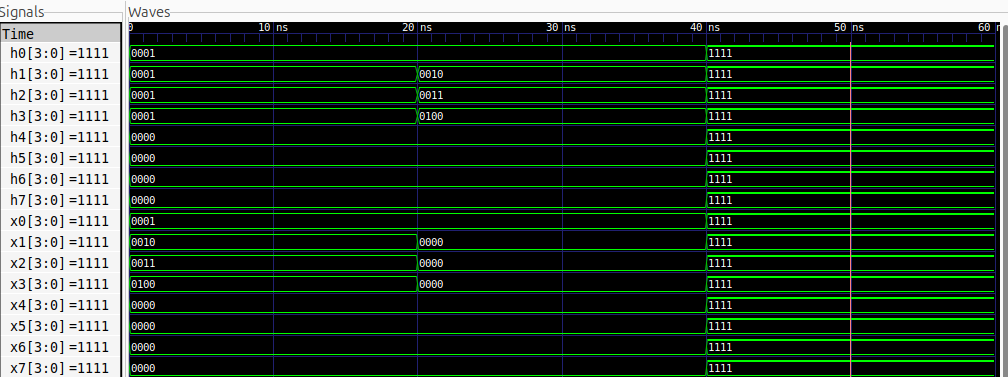
\includegraphics[width=0.9\textwidth]{1.png}
      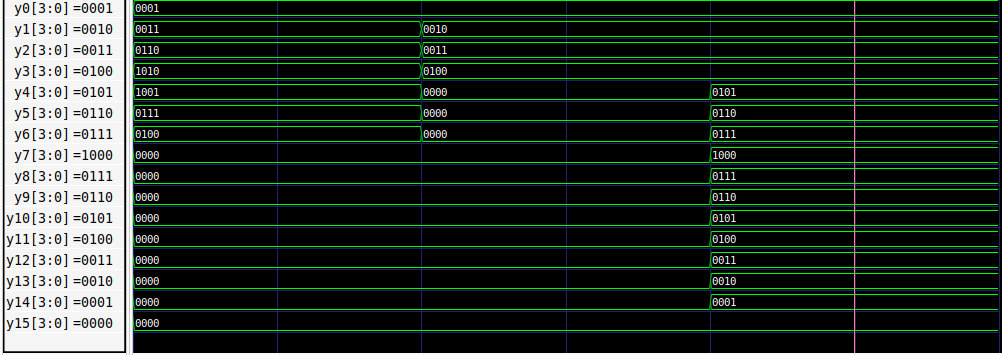
\includegraphics[width=0.9\textwidth]{2.png}
    \caption{Timing diagram showing convolution outputs for different input patterns}
    \label{fig:conv_timing}
\end{figure}

\section{Question 2: 8-bit Full Adder Using Loop Statements}

\subsection{Detailed Approach}
\begin{enumerate}
    \item The design implements an 8-bit adder using a generate loop.
    \item It instantiates 8 full adder modules in a cascaded fashion.
    \item The generate block creates a ripple-carry adder structure.
    \item First full adder handles the carry-in input specially.
    \item Subsequent adders connect to previous carry-out.
    \item Uses a hierarchical design with a basic full adder module.
    \item The loop variable 'i' creates unique instances for each bit.
    \item Internal carry wires connect adjacent full adders.
    \item Final carry-out comes from the last full adder.
    \item Demonstrates parameterized design using Verilog generate.
\end{enumerate}

\subsection{Code Explanation}
Key points about the implementation:
\begin{itemize}
    \item Uses hierarchical design with 1-bit full adder module
    \item Generate loop creates 8 instances of full adder
    \item Special handling for first adder's carry-in
    \item Internal carry chain connects adjacent adders
    \item Clean separation of module definition and instantiation
    \item Demonstrates Verilog's generate construct
    \item Efficient parameterized design
    \item Easy to scale to different bit widths
\end{itemize}

\begin{tcolorbox}[title=8-bit Adder Module Code, breakable]
\begin{lstlisting}[language=Verilog]
module full_adder (
    input  a, b, cin,
    output sum, cout
);
    assign sum = a ^ b ^ cin;
    assign cout = (a & b) | (b & cin) | (a & cin);
endmodule

module adder_8bit (
    input  [7:0] A, B,
    input        Cin,
    output [7:0] Sum,
    output       Cout
);
    wire [7:0] carry;
    
    genvar i;
    generate
        for (i = 0; i < 8; i = i + 1) begin : full_adder_loop
            if (i == 0) begin
                full_adder FA (
                    .a(A[i]),
                    .b(B[i]),
                    .cin(Cin),
                    .sum(Sum[i]),
                    .cout(carry[i])
                );
            end else begin
                full_adder FA (
                    .a(A[i]),
                    .b(B[i]),
                    .cin(carry[i-1]),
                    .sum(Sum[i]),
                    .cout(carry[i])
                );
            end
        end
    endgenerate
    
    assign Cout = carry[7];
endmodule
\end{lstlisting}
\end{tcolorbox}

\subsection{Testbench}
Key testbench features:
\begin{itemize}
    \item Tests four different addition scenarios
    \item Includes basic, carry-in, and overflow cases
    \item Verifies both sum and carry-out outputs
    \item 10ns delay between test cases
    \item Uses binary literals for input values
    \item Clear display messages for each test
\end{itemize}

\begin{tcolorbox}[title=8-bit Adder Testbench, breakable]
\begin{lstlisting}[language=Verilog]
`timescale 1ns / 1ps

module tb_adder_8bit;
    reg  [7:0] A, B;
    reg        Cin;
    wire [7:0] Sum;
    wire       Cout;

    adder_8bit uut (
        .A(A),
        .B(B),
        .Cin(Cin),
        .Sum(Sum),
        .Cout(Cout)
    );

    initial begin
        $dumpfile("adder_8bit.vcd");
        $dumpvars(0, tb_adder_8bit);

        // Test 1: Basic Addition
        A = 8'b00001111; B = 8'b00000001; Cin = 0; #10;

        // Test 2: With Carry-in
        A = 8'b11110000; B = 8'b00001111; Cin = 1; #10;

        // Test 3: Max values
        A = 8'b11111111; B = 8'b11111111; Cin = 0; #10;

        // Test 4: Random pattern
        A = 8'b10101010; B = 8'b01010101; Cin = 0; #10;

        $display("Simulation complete.");
        $finish;
    end
endmodule
\end{lstlisting}
\end{tcolorbox}

\subsection{Timing Diagram}
\begin{figure}[H]
    \centering
    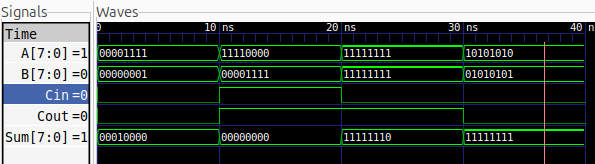
\includegraphics[width=0.9\textwidth]{3.png}
    \caption{Timing diagram showing 8-bit adder operation with carry propagation}
    \label{fig:adder_timing}
\end{figure}

\section{Question 3: 4-bit Ripple Carry Adder Using NAND Gates}

\subsection{Detailed Approach}
\begin{enumerate}
    \item Implements a 4-bit adder using only 2-input NAND gates.
    \item Each NAND gate has 1ns propagation delay.
    \item Hierarchical design with basic logic gates built from NANDs.
    \item Includes NOT, AND, OR, and XOR implementations using NANDs.
    \item Full adder constructed from these basic gates.
    \item Ripple carry adder chains 4 full adders together.
    \item Carry propagates through each stage sequentially.
    \item Demonstrates universal gate implementation.
    \item Shows gate-level design with precise timing.
    \item Testbench verifies correct operation with timing checks.
\end{enumerate}

\subsection{Code Explanation}
Key points about the implementation:
\begin{itemize}
    \item All logic gates derived from NAND gates
    \item Precise 1ns delay per NAND gate
    \item Hierarchical design from basic gates to full adder
    \item Ripple carry structure with explicit carry propagation
    \item Demonstrates universal gate property of NAND
    \item Gate-level implementation shows actual hardware
    \item Clear separation of different logic functions
    \item Includes all necessary intermediate wires
\end{itemize}

\begin{tcolorbox}[title=NAND-based Adder Code, breakable]
\begin{lstlisting}[language=Verilog]
`timescale 1ns / 1ps

module nand2(input a, b, output y);
    assign #1 y = ~(a & b);
endmodule

module not_nand(input a, output y);
    nand2 n1(a, a, y);
endmodule

module and_nand(input a, b, output y);
    wire t;
    nand2 n1(a, b, t);
    nand2 n2(t, t, y);
endmodule

module or_nand(input a, b, output y);
    wire na, nb;
    not_nand n1(a, na);
    not_nand n2(b, nb);
    nand2 n3(na, nb, y);
endmodule

module xor_nand(input a, b, output y);
    wire t1, t2, t3;
    nand2 n1(a, b, t1);
    nand2 n2(a, t1, t2);
    nand2 n3(b, t1, t3);
    nand2 n4(t2, t3, y);
endmodule

module full_adder_nand(input a, b, cin, output sum, cout);
    wire axb, ab, bc, ac, t;
    xor_nand x1(a, b, axb);
    xor_nand x2(axb, cin, sum);
    and_nand a1(a, b, ab);
    and_nand a2(b, cin, bc);
    and_nand a3(a, cin, ac);
    or_nand o1(ab, bc, t);
    or_nand o2(t, ac, cout);
endmodule

module ripple_carry_adder_4bit(
    input  [3:0] A, B,
    input        Cin,
    output [3:0] Sum,
    output       Cout
);
    wire c1, c2, c3;
    
    full_adder_nand fa0(A[0], B[0], Cin,  Sum[0], c1);
    full_adder_nand fa1(A[1], B[1], c1,   Sum[1], c2);
    full_adder_nand fa2(A[2], B[2], c2,   Sum[2], c3);
    full_adder_nand fa3(A[3], B[3], c3,   Sum[3], Cout);
endmodule
\end{lstlisting}
\end{tcolorbox}

\subsection{Testbench}
Key testbench features:
\begin{itemize}
    \item Tests five different addition scenarios
    \item Includes overflow, simple, and random cases
    \item 100ns delay to observe gate delays
    \item Verifies correct timing behavior
    \item Tests all bits and carry chains
    \item Includes edge cases and typical patterns
\end{itemize}

\begin{tcolorbox}[title=NAND Adder Testbench, breakable]

\begin{lstlisting}[language=Verilog]
`timescale 1ns / 1ps

module tb_ripple_adder;
    reg  [3:0] A, B;
    reg        Cin;
    wire [3:0] Sum;
    wire       Cout;

    ripple_carry_adder_4bit uut (
        .A(A), .B(B), .Cin(Cin),
        .Sum(Sum), .Cout(Cout)
    );
    initial begin
        $dumpfile("ripple_adder.vcd");
        $dumpvars(0, tb_ripple_adder);

        // Test 1: 15 + 15 + 1 = 31 (Overflow)
        A = 4'b1111; B = 4'b1111; Cin = 1; #100;

        // Test 2: 1 + 2 = 3
        A = 4'b0001; B = 4'b0010; Cin = 0; #100;

        // Test 3: Alternating bits with Cin
        A = 4'b1010; B = 4'b0101; Cin = 1; #100;

        // Test 4: All zeros
        A = 4'b0000; B = 4'b0000; Cin = 0; #100;

        // Test 5: Random mix
        A = 4'b1001; B = 4'b0110; Cin = 1; #100;
        $finish;
    end
endmodule
\end{lstlisting}
\end{tcolorbox}

\subsection{Timing Diagram}
\begin{figure}[H]
    \centering
    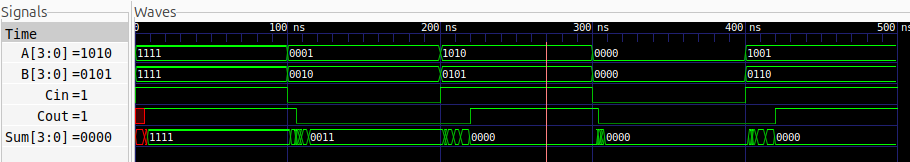
\includegraphics[width=0.9\textwidth]{4.png}
    \caption{Timing diagram showing ripple carry propagation in 4-bit adder}
    \label{fig:ripple_timing}
\end{figure}
\begin{center}
\fbox{\url{https://github.com/Dhawal24112006/EE1501.git}}
\end{center}
\end{document}
